% ============================================================================
% SERGE — Final Report
% SE618 Logistic Case Study Analysis — Semester 2/2025
% ============================================================================

\documentclass[12pt,a4paper]{report}

% ── Encoding ─────────────────────────────────────────────────────────
\usepackage[utf8]{inputenc}
\usepackage[T1]{fontenc}

% ── Layout ───────────────────────────────────────────────────────────
\usepackage[top=2.2cm, bottom=2.2cm, left=2.2cm, right=2.2cm]{geometry}
\usepackage{setspace}
\setstretch{1.1}
\setlength{\parindent}{0pt}
\setlength{\parskip}{0.35em}

% ── Fonts ────────────────────────────────────────────────────────────
\usepackage{lmodern}
\usepackage{microtype}
\usepackage{ragged2e}

% ── Paragraph robustness ─────────────────────────────────────────────
\sloppy
\emergencystretch=1em
\hbadness=10000

% ── Colors ───────────────────────────────────────────────────────────
\usepackage[dvipsnames]{xcolor}
\definecolor{scblue}{HTML}{1E40AF}
\definecolor{scdark}{HTML}{1E3A8A}
\definecolor{scaccent}{HTML}{F59E0B}
\definecolor{lightgray}{HTML}{F5F5F5}

% ── Headers and footers ──────────────────────────────────────────────
\usepackage{fancyhdr}
\pagestyle{fancy}
\fancyhf{}
\fancyhead[L]{\leftmark}
\fancyhead[R]{\thepage}
\fancyfoot[C]{\textcolor{scblue}{SERGE --- Supply Chain Agent}}
\renewcommand{\headrulewidth}{0.4pt}
\renewcommand{\footrulewidth}{0.4pt}

% ── Titles ───────────────────────────────────────────────────────────
\usepackage{titlesec}
\titleformat{\chapter}[hang]
  {\normalfont\Large\bfseries\color{scblue}}
  {\thechapter.}{14pt}{}
\titlespacing*{\chapter}{0pt}{-15pt}{8pt}
\titleformat{\section}
  {\normalfont\large\bfseries\color{scdark}}
  {\thesection}{0.7em}{}
\titlespacing*{\section}{0pt}{10pt}{4pt}
\titleformat{\subsection}
  {\normalfont\normalsize\bfseries}
  {\thesubsection}{0.6em}{}
\titlespacing*{\subsection}{0pt}{7pt}{2pt}

% ── Graphics ─────────────────────────────────────────────────────────
\usepackage{graphicx}
\usepackage{float}
\usepackage{subcaption}
\graphicspath{{images/}{figures/}}

% ── Tables ───────────────────────────────────────────────────────────
\usepackage{booktabs}
\usepackage{tabularx}
\usepackage{longtable}
\usepackage{array}
\usepackage{colortbl}

% ── Lists ────────────────────────────────────────────────────────────
\usepackage{enumitem}

% ── Listings ─────────────────────────────────────────────────────────
\usepackage{listings}
\lstset{
  basicstyle=\ttfamily\small,
  backgroundcolor=\color{lightgray},
  frame=single,
  rulecolor=\color{scblue},
  keywordstyle=\color{scblue}\bfseries,
  commentstyle=\color{gray}\itshape,
  numbers=left,
  numberstyle=\tiny\color{gray},
  breaklines=true,
  showstringspaces=false,
  tabsize=2,
  captionpos=b,
}

% ── Boxes ────────────────────────────────────────────────────────────
\usepackage[most]{tcolorbox}

% ── Hyperref ─────────────────────────────────────────────────────────
\usepackage[hyphens,spaces,obeyspaces]{url}
\usepackage{hyperref}
\hypersetup{
  colorlinks=true,
  linkcolor=scblue,
  urlcolor=scblue,
  citecolor=scblue,
  pdftitle={SERGE - Final Report},
  pdfauthor={Grignola, Schmitt, Tellus, Schwarz},
}

% ── Glossary ─────────────────────────────────────────────────────────
\usepackage[acronym,toc,nopostdot]{glossaries}
\makeglossaries

% ── TikZ ─────────────────────────────────────────────────────────────
\usepackage{tikz}
\usetikzlibrary{shapes,arrows,positioning,fit,backgrounds}
\pgfdeclarelayer{background}
\pgfsetlayers{background,main}

% ── Columns ──────────────────────────────────────────────────────────
\newcolumntype{L}[1]{>{\raggedright\arraybackslash}p{#1}}
\newcolumntype{C}[1]{>{\centering\arraybackslash}p{#1}}

% ============================================================================
% GLOSSARY ENTRIES
% ============================================================================

\newacronym{srm}{SRM}{Supplier Relationship Management}
\newacronym{wms}{WMS}{Warehouse Management System}
\newacronym{oms}{OMS}{Order Management System}
\newacronym{tms}{TMS}{Transport Management System}
\newacronym{mcp}{MCP}{Model Context Protocol}
\newacronym{llm}{LLM}{Large Language Model}
\newacronym{ai}{AI}{Artificial Intelligence}
\newacronym{api}{API}{Application Programming Interface}
\newacronym{po}{PO}{Purchase Order}
\newacronym{sdk}{SDK}{Software Development Kit}

\newglossaryentry{react}{
  name={ReAct},
  description={Reasoning and Acting; an agent paradigm that interleaves a reasoning step (thought) and an action step (tool call) in a single loop}
}
\newglossaryentry{boundedcontext}{
  name={bounded context},
  description={In Domain-Driven Design, a coherent region of a software system within which a single ubiquitous language applies; inter-context references are carried by stable identifiers rather than by object references}
}

% ============================================================================
% DOCUMENT
% ============================================================================

\begin{document}

% ── Cover ────────────────────────────────────────────────────────────
% ============================================================================
% COVER PAGE
% ============================================================================

\begin{titlepage}
    \newgeometry{left=2.5cm, right=2.5cm, top=2cm, bottom=2cm}

    \noindent
    
\includegraphics[height=1.8cm]{siitlogo.png}

    \vspace{2.5cm}

    \noindent
    {\large SE618 Logistic Case Study Analysis}\\[0.3cm]
    {\large Academic Year 2025--2026, Semester 2}

    \vspace{2.5cm}

    \noindent
    {\fontsize{56}{68}\selectfont\bfseries\color{scblue} SERGE}\\[0.4cm]
    {\LARGE An AI Agent for Cross-System}\\[0.15cm]
    {\LARGE Supply Chain Diagnostics via MCP}

    \vspace{1.0cm}

    \noindent
    {\large Final Report}\\[0.3cm]
    {\normalsize Design, Implementation, and Empirical Evaluation}

    \vfill

    \noindent
    {\large\bfseries Authors}\\[0.3cm]
    Gauthier Schmitt \hfill 6822807466\\
    Louis Grignola  \hfill 6822807516\\
    Matteo Schwarz  \hfill 6822807557\\
    Ma\"el Tellus    \hfill 6822807532

    \vspace{1.0cm}

    \noindent
    {\large\bfseries Supervisor}\\[0.15cm]
    Ajarn Warut

    \vspace{0.8cm}

    \noindent
    {\small School of Manufacturing Systems and Mechanical Engineering}\\
    {\small Sirindhorn International Institute of Technology --- Thammasat University}\\[0.4cm]
    {\small April 2026}

    \restoregeometry
\end{titlepage}


% ── Front matter ─────────────────────────────────────────────────────
\pagenumbering{roman}

\tableofcontents
\clearpage

\listoffigures
\clearpage

\listoftables
\clearpage

% ── Body ─────────────────────────────────────────────────────────────
\pagenumbering{arabic}

% ============================================================================
% CHAPTER 1 — INTRODUCTION
% ============================================================================

\chapter{Introduction}
\label{ch:intro}

\section{The Problem}

Supply chains run on four enterprise systems: \gls{srm} (procurement), \gls{wms} (inventory), \gls{oms} (sales), \gls{tms} (shipping). These systems come from different vendors and do not talk to each other. A GEODIS survey reports only 6\% of companies achieve full visibility across them~\cite{geodis2024}; operations managers spend 15 to 30 minutes per investigation manually stitching data from three or four interfaces~\cite{aws2024sync,omniful2026}.

Most cross-system questions are blocked by this fragmentation: \emph{why is this order late?}, \emph{which customers are at risk if product X runs out?}, \emph{is the chosen carrier appropriate for that product?}

\section{The Question}

\emph{Can an AI agent with read-only access to the four systems answer realistic operational questions at human-level factual accuracy, while significantly reducing investigation time?}

\section{SERGE}

We build \textbf{SERGE}, a read-only agent that sits over the four supply chain systems via the Model Context Protocol~\cite{mcp2024}. A simulated B2B mango distributor is used as the target domain; its four systems are exposed as 35 read-only \gls{mcp} tools. Claude Code acts as the reasoning agent, invoked from the user's desktop client.

The system is evaluated on 27 scenarios spanning five complexity levels (L1 trivial to L5 expert). Each scenario is run three times, judged by a separate \gls{llm} on four dimensions (factual accuracy, completeness, hallucination, reasoning), and aggregated. Two passes are reported: a baseline and a refined run after one iteration cycle.

\section{Contributions}

\begin{enumerate}
    \item A plug-and-play \gls{mcp} architecture for supply chain systems, agent-agnostic by design.
    \item A read-only diagnostic agent pattern, complementary to the optimisation-centric supply chain \gls{ai} literature.
    \item An \gls{llm}-as-judge methodology with an explicit \emph{flexible-on-form, strict-on-facts} principle and a structured failure taxonomy.
    \item A reusable benchmark of 27 scenarios at five complexity levels.
\end{enumerate}

\section{Headline Results}

Refined pass (Run~2): 94\% pass rate over 81 evaluations, weighted score 4.84/5.0, \textbf{zero hallucinations}, 100\% pass on L4 (complex cross-system) scenarios. Resolution time averages about 13\,s on L1 and 72\,s on L5.

\section{Report Map}

Chapter~\ref{ch:background}: background on \gls{llm}s, agents, and \gls{mcp}. Chapter~\ref{ch:relwork}: related work. Chapter~\ref{ch:modelisation}: the modelled business, the entity model, and how the dataset was seeded. Chapter~\ref{ch:architecture}: the agent--\gls{mcp}--backend stack. Chapter~\ref{ch:methodology}: evaluation methodology. Chapter~\ref{ch:scenarios}: the 27 scenarios. Chapter~\ref{ch:results}: empirical results, including the refinement cycle. Chapter~\ref{ch:discussion}: discussion. Chapter~\ref{ch:conclusion}: conclusion.

% ============================================================================
% CHAPTER 2 — BACKGROUND
% ============================================================================

\chapter{Background}
\label{ch:background}

\section{Large Language Models}

A \gls{llm} is a deep neural network trained on very large text corpora. All modern \gls{llm}s are built on the \textbf{Transformer} architecture~\cite{vaswani2017attention}. Loss scales predictably with model size, data size, and compute~\cite{kaplan2020scaling,hoffmann2022chinchilla}; capabilities such as multi-step reasoning and tool use \emph{emerge} past capability thresholds rather than improving linearly~\cite{wei2022emergent}. In April 2026 the practical models are Claude~4.5, GPT-5, Llama~4, and Mistral Large~3. This work uses Claude Sonnet through the Claude Code client.

A \gls{llm} on its own is a text-to-text function: no memory, no tools, no ability to act. For supply chain diagnostics---which require reading state from multiple sources---the \gls{llm} must be embedded in a larger system that provides tools and a reasoning loop. That system is the agent.

\section{AI Agents}

An \textbf{agent} wraps an \gls{llm} with (i) a set of tools it can call, (ii) a mechanism to observe the tool result, and (iii) a loop that decides what to call next and when to stop~\cite{weng2023agents}. The seminal formulation is \gls{react}~\cite{yao2023react}: the \gls{llm} alternates reasoning steps and tool calls until it emits a terminal response.

The agent used here, Claude Code~\cite{anthropic2025howccworks}, goes beyond a plain \gls{react} loop: extended thinking is built in, sub-agent spawning is available, reusable workflows can be loaded on demand, and context is actively managed~\cite{anthropic2025contextengineering}. Tool description quality is the dominant factor in tool-call reliability~\cite{anthropic2025writingtools,schick2023toolformer,patil2024gorilla}, a point we return to in the architecture chapter.

\section{Model Context Protocol}

Without a standard integration layer, every agent-system pair needs bespoke code; with $N$ agents and $M$ systems the integration matrix has $N \times M$ cells. The \gls{mcp}~\cite{mcp2024,mcpspec}, introduced by Anthropic in November~2024, collapses this matrix to $N + M$: each agent and each system implements \gls{mcp} once and all combinations work. Primitives are \emph{tools} (callable functions with typed parameters), \emph{resources} (readable data), and \emph{prompts} (templates); transports are \texttt{stdio} (subprocess) or HTTP. SERGE uses tools only, over \texttt{stdio}.

\gls{mcp} is the right glue for SERGE for three reasons: it is agent-agnostic (swap Claude for any \gls{mcp} client without touching the backend), typed and self-describing (new agents connect without extra configuration), and trivial to deploy locally (no network services to run).

% ============================================================================
% CHAPTER 3 — RELATED WORK
% ============================================================================

\chapter{Related Work}
\label{ch:relwork}

\section{AI Agents for Supply Chain}

Multi-agent \gls{llm} systems have been shown to reduce the bullwhip effect in simulation~\cite{jannelli2024agentic}. Generative planning has been deployed at industrial scale by JD.com (SCPA)~\cite{yin2025scpa}. Knowledge-graph query agents have been applied to disruption monitoring~\cite{almahri2026disruption}, and multi-agent retrieval pipelines have been used to ingest unstructured supply chain communications~\cite{zhang2025rag}. All four systems aim at autonomous action. SERGE takes the complementary read-only diagnostic position: an agent that reads current state and explains it, before anything is written back.

A systematic review of 98 peer-reviewed studies~\cite{gaisc2025systematic} observes that about 45\% of published \gls{ai}-for-supply-chain work does not fully specify its architecture. The field is still methodologically young.

\section{LLM-as-Judge}

Zheng et~al.~\cite{zheng2023judge} introduced the \gls{llm}-as-judge framework with MT-Bench and Chatbot Arena, reporting over 80\% agreement with human raters. Follow-up surveys~\cite{gu2024judgesurvey,li2024judgessurvey} catalogue common biases (position, verbosity, self-enhancement) and their mitigations. Shankar et~al.~\cite{shankar2024validators} examine rubric design and alignment with human judgement. Our methodology (Chapter~\ref{ch:methodology}) uses pointwise judging with a domain-specific rubric and adds an explicit \emph{flexible-on-form} rule after observing the strictness failure mode in our own baseline run.

\section{Gaps Addressed}

Four gaps identified in our Week~3 state-of-the-art review motivate this work: (1)~no standardised supply chain agent benchmark, (2)~no plug-and-play architecture connecting supply chain systems to agents, (3)~read-only diagnostic agents underexplored, (4)~no supply-chain-specific \gls{llm}-as-judge rubric. SERGE addresses gaps 2--4 directly; the 27 scenarios released with this work contribute to gap~1.

% ============================================================================
% CHAPTER 4 — BUSINESS AND SUPPLY CHAIN MODELISATION
% ============================================================================

\chapter{Business and Supply Chain Modelisation}
\label{ch:modelisation}

\section{The Business: Siam Mango Co.}

Siam Mango Co.\ is a fictional small B2B mango distributor in Bangkok. It sources from 5 Thai farms, stores in 1 warehouse (Bang Na), sells 5 fresh and 3 processed products to 12 business customers (hotels, supermarkets, food halls), and delivers through 3 carriers (1 ground, 2 refrigerated). The domain is small enough to audit manually and rich enough to exercise four realistic constraints: perishability (fresh shelf life 3--10 days), cold chain (refrigerated products require refrigerated carriers), supplier reliability (0--100\% on-time in the data), and multi-sourcing (most products available from two farms at different costs).

\section{Four Bounded Contexts}

The four supply chain systems map to four bounded contexts in the Domain-Driven Design sense: each has its own ubiquitous language and its own state; cross-context references are carried by stable identifiers.

\begin{table}[H]
    \centering\small
    \begin{tabularx}{\textwidth}{|l|l|X|}
        \hline
        \rowcolor{lightgray}
        \textbf{System} & \textbf{Domain} & \textbf{Entities} \\
        \hline
        \gls{srm} & Procurement & Supplier, SupplierProduct, SupplierOrder \\
        \hline
        \gls{wms} & Inventory   & Product, Warehouse, InventoryRecord, StockMovement \\
        \hline
        \gls{oms} & Sales       & Customer, CustomerOrder \\
        \hline
        \gls{tms} & Shipping    & Carrier, Shipment, TrackingEvent \\
        \hline
    \end{tabularx}
    \caption{Supply chain systems and their entities.}
    \label{tab:systems}
\end{table}

\section{Entity Model}

Figure~\ref{fig:classdiagram} shows the conceptual class diagram. Solid arrows are associations within a context; dashed arrows are cross-context references carried by identifier. One design point is worth calling out: prices are not duplicated on order lines. A \texttt{SupplierProduct} bridge entity carries the purchase cost; sale prices live on the \texttt{Product} entity. Order lines reference a product-level entity and a quantity---nothing else. This removes a whole class of ``price on line vs price in catalogue'' inconsistencies and sharpens the domain language the agent reads in its system prompt.

\begin{figure}[H]
    \centering
    \resizebox{\textwidth}{!}{% ============================================================================
% UML CLASS DIAGRAM — SERGE Domain Model
% Uses tabular-in-rect nodes (no rectangle split — avoids header/body overlap).
% Canvas sized to ~textwidth so resizebox barely scales.
% ============================================================================
\newcommand{\umlclass}[2]{%
  \begin{tabular}{@{}l@{}}\bfseries #1\\\hline #2\end{tabular}%
}
\newcommand{\umlenum}[2]{%
  \begin{tabular}{@{}c@{}}\scriptsize$\langle\langle$enum$\rangle\rangle$\\\bfseries #1\\\hline #2\end{tabular}%
}

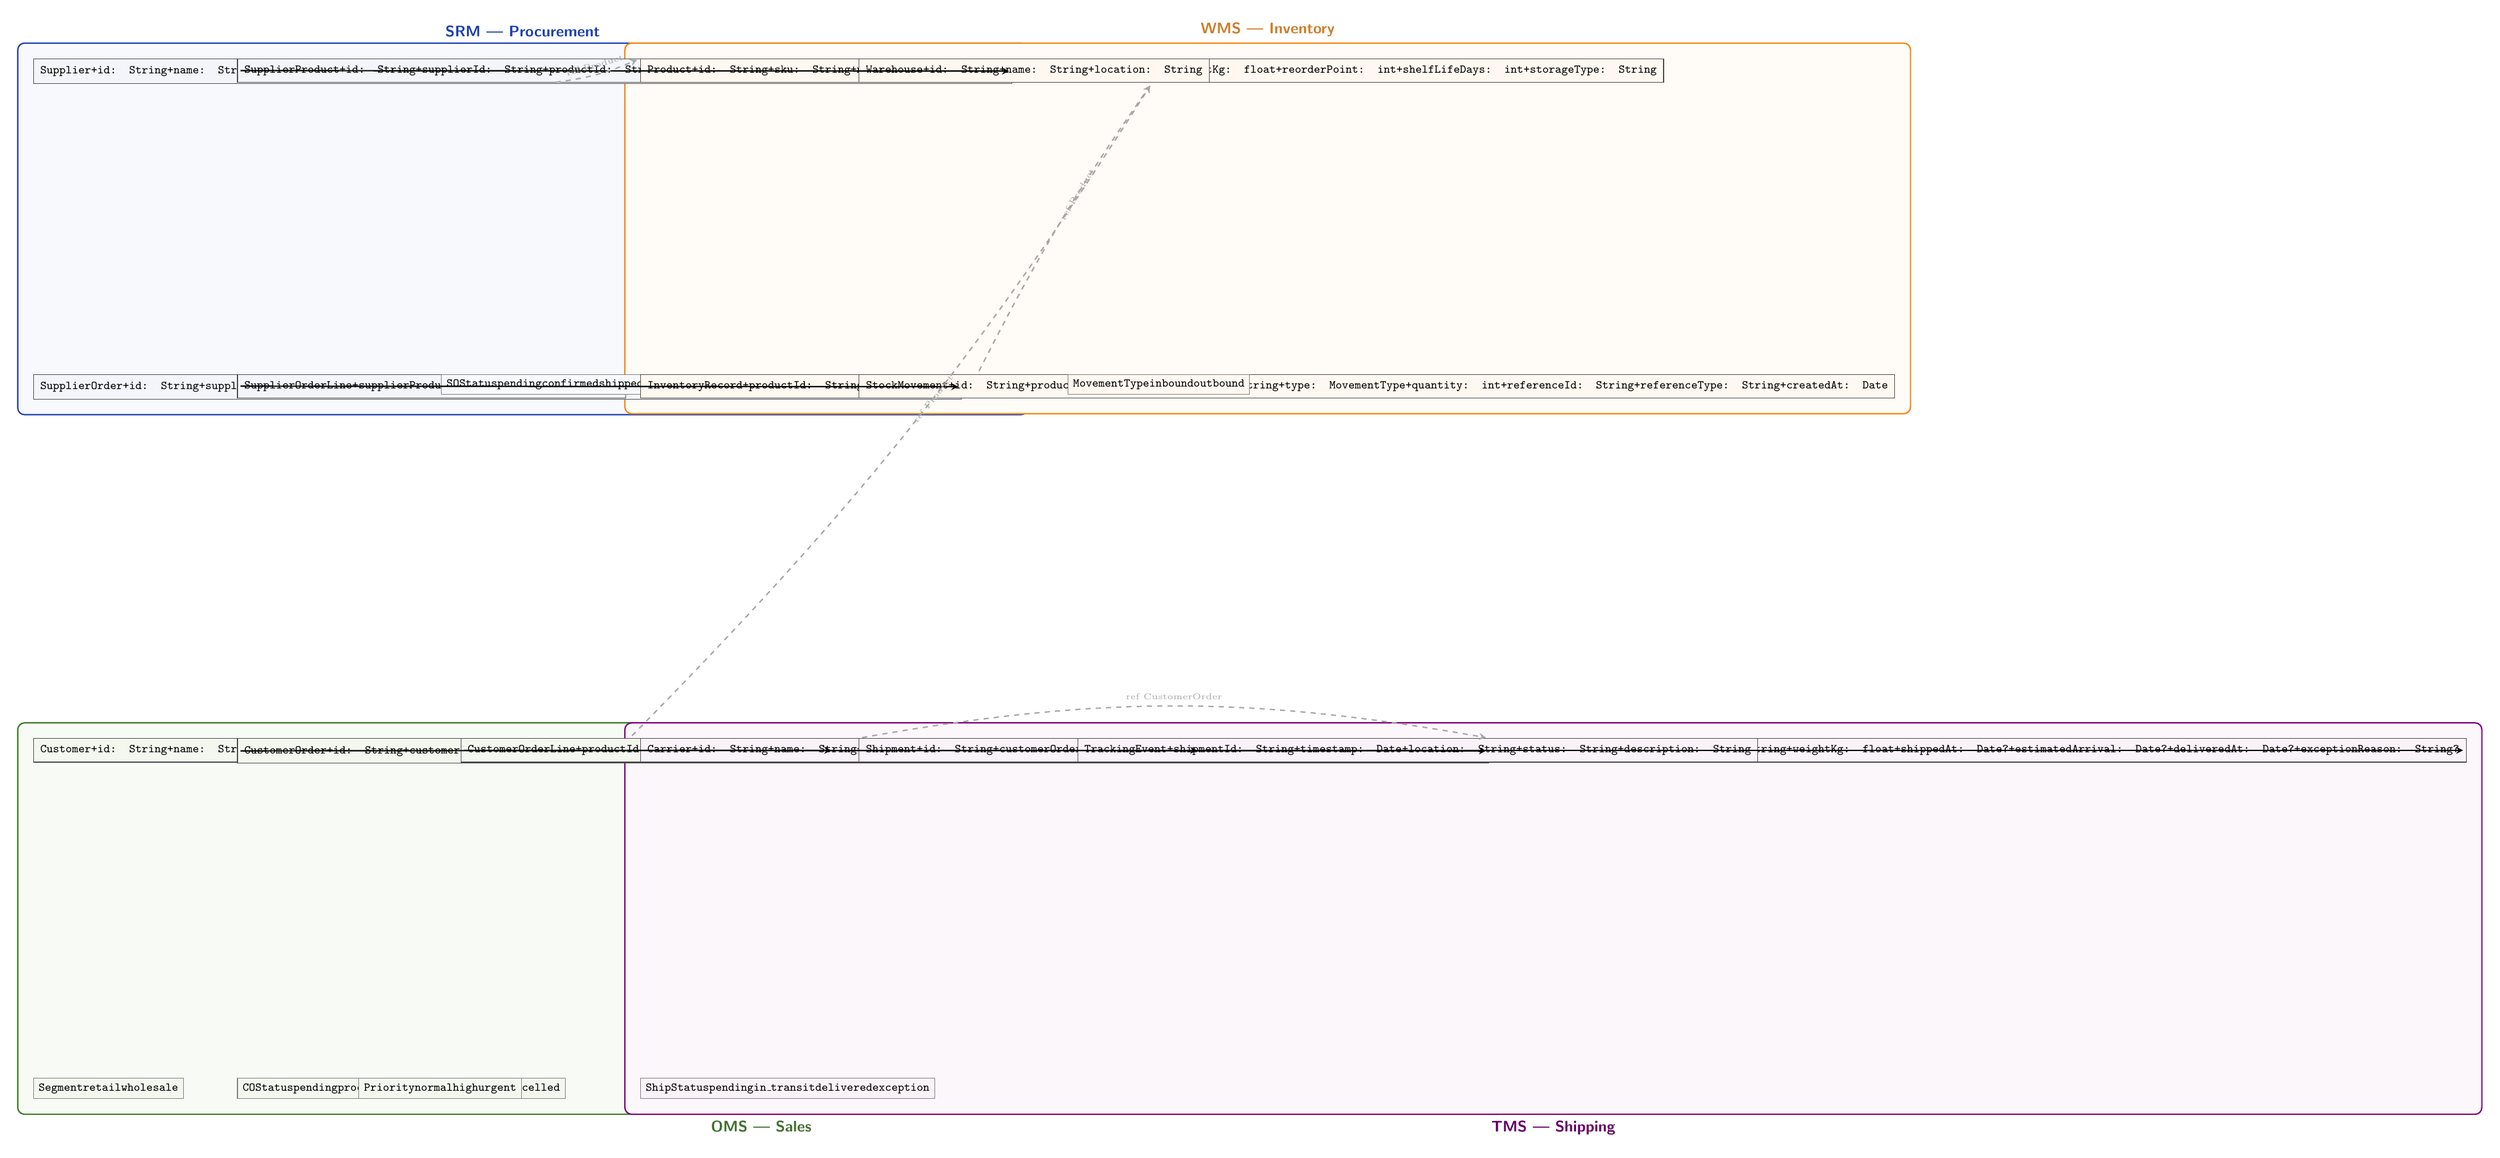
\begin{tikzpicture}[
    every node/.style={font=\ttfamily\scriptsize},
    cls/.style={rectangle, draw=black!70, inner sep=4pt, anchor=north west},
    enm/.style={rectangle, draw=black!50, inner sep=3pt, anchor=north west},
    zone/.style={rounded corners, draw, thick, inner sep=9pt, font=\sffamily\footnotesize\bfseries},
    rel/.style={->, >=stealth, thick, shorten >=2pt, shorten <=2pt},
    xrel/.style={->, >=stealth, dashed, thick, gray!70, shorten >=2pt, shorten <=2pt},
]

% ================= SRM — top left =================
\node[cls, fill=scblue!5] (Supplier) at (0, 22) {\umlclass{Supplier}{%
+id: String\\
+name: String\\
+region: String\\
+contact: String\\
+leadTimeDays: int\\
+rating: float\\
+paymentTerms: String\\
+productCategories: []String}};

\node[cls, fill=scblue!5] (SupplierProduct) at (4.2, 22) {\umlclass{SupplierProduct}{%
+id: String\\
+supplierId: String\\
+productId: String\\
+name: String\\
+unitCost: float}};

\node[cls, fill=scblue!5] (SupplierOrder) at (0, 15.5) {\umlclass{SupplierOrder}{%
+id: String\\
+supplierId: String\\
+status: SOStatus\\
+orderDate: Date\\
+expectedDelivery: Date\\
+actualDelivery: Date?\\
+lines: []SOLine}};

\node[cls, fill=scblue!5] (SOLine) at (4.2, 15.5) {\umlclass{SupplierOrderLine}{%
+supplierProductId: String\\
+quantity: int}};

\node[enm, fill=scblue!3] (SOStatus) at (8.4, 15.5) {\umlenum{SOStatus}{%
pending\\
confirmed\\
shipped\\
received\\
cancelled}};

\begin{pgfonlayer}{background}
    \node[zone, draw=scblue, fill=scblue!3,
          fit=(Supplier)(SupplierProduct)(SupplierOrder)(SOLine)(SOStatus),
          label={[scblue,font=\sffamily\bfseries\small]above:SRM --- Procurement}] (SRMzone) {};
\end{pgfonlayer}

% ================= WMS — top right =================
\node[cls, fill=BurntOrange!5] (Product) at (12.5, 22) {\umlclass{Product}{%
+id: String\\
+sku: String\\
+name: String\\
+category: String\\
+unitPrice: float\\
+weightKg: float\\
+reorderPoint: int\\
+shelfLifeDays: int\\
+storageType: String}};

\node[cls, fill=BurntOrange!5] (Warehouse) at (17, 22) {\umlclass{Warehouse}{%
+id: String\\
+name: String\\
+location: String}};

\node[cls, fill=BurntOrange!5] (InventoryRecord) at (12.5, 15.5) {\umlclass{InventoryRecord}{%
+productId: String\\
+warehouseId: String\\
+quantity: int\\
+reserved: int\\
+lastUpdated: Date}};

\node[cls, fill=BurntOrange!5] (StockMovement) at (17, 15.5) {\umlclass{StockMovement}{%
+id: String\\
+productId: String\\
+warehouseId: String\\
+type: MovementType\\
+quantity: int\\
+referenceId: String\\
+referenceType: String\\
+createdAt: Date}};

\node[enm, fill=BurntOrange!5] (MovementType) at (21.3, 15.5) {\umlenum{MovementType}{%
inbound\\
outbound}};

\begin{pgfonlayer}{background}
    \node[zone, draw=BurntOrange, fill=BurntOrange!3,
          fit=(Product)(Warehouse)(InventoryRecord)(StockMovement)(MovementType),
          label={[BurntOrange!80!black,font=\sffamily\bfseries\small]above:WMS --- Inventory}] (WMSzone) {};
\end{pgfonlayer}

% ================= OMS — bottom left =================
\node[cls, fill=OliveGreen!5] (Customer) at (0, 8) {\umlclass{Customer}{%
+id: String\\
+name: String\\
+company: String\\
+segment: Segment\\
+region: String\\
+address: String\\
+deliveryZone: String}};

\node[cls, fill=OliveGreen!5] (CustomerOrder) at (4.2, 8) {\umlclass{CustomerOrder}{%
+id: String\\
+customerId: String\\
+status: COStatus\\
+orderDate: Date\\
+requiredDate: Date\\
+shippedDate: Date?\\
+deliveredDate: Date?\\
+priority: Priority\\
+notes: String?\\
+lines: []COLine}};

\node[cls, fill=OliveGreen!5] (COLine) at (8.8, 8) {\umlclass{CustomerOrderLine}{%
+productId: String\\
+quantity: int}};

\node[enm, fill=OliveGreen!5] (Segment) at (0, 1) {\umlenum{Segment}{%
retail\\
wholesale}};

\node[enm, fill=OliveGreen!5] (COStatus) at (4.2, 1) {\umlenum{COStatus}{%
pending\\
processing\\
shipped\\
delivered\\
cancelled}};

\node[enm, fill=OliveGreen!5] (Priority) at (6.7, 1) {\umlenum{Priority}{%
normal\\
high\\
urgent}};

\begin{pgfonlayer}{background}
    \node[zone, draw=OliveGreen, fill=OliveGreen!3,
          fit=(Customer)(CustomerOrder)(COLine)(COStatus)(Priority)(Segment),
          label={[OliveGreen!80!black,font=\sffamily\bfseries\small]below:OMS --- Sales}] (OMSzone) {};
\end{pgfonlayer}

% ================= TMS — bottom right =================
\node[cls, fill=Purple!5] (Carrier) at (12.5, 8) {\umlclass{Carrier}{%
+id: String\\
+name: String\\
+type: String\\
+costPerKg: float\\
+avgTransitDays: int}};

\node[cls, fill=Purple!5] (Shipment) at (17, 8) {\umlclass{Shipment}{%
+id: String\\
+customerOrderId: String\\
+carrierId: String\\
+status: ShipStatus\\
+trackingNumber: String\\
+origin: String\\
+destination: String\\
+weightKg: float\\
+shippedAt: Date?\\
+estimatedArrival: Date?\\
+deliveredAt: Date?\\
+exceptionReason: String?}};

\node[cls, fill=Purple!5] (TrackingEvent) at (21.5, 8) {\umlclass{TrackingEvent}{%
+shipmentId: String\\
+timestamp: Date\\
+location: String\\
+status: String\\
+description: String}};

\node[enm, fill=Purple!5] (ShipStatus) at (12.5, 1) {\umlenum{ShipStatus}{%
pending\\
in\_transit\\
delivered\\
exception}};

\begin{pgfonlayer}{background}
    \node[zone, draw=Purple, fill=Purple!3,
          fit=(Carrier)(Shipment)(TrackingEvent)(ShipStatus),
          label={[Purple!80!black,font=\sffamily\bfseries\small]below:TMS --- Shipping}] (TMSzone) {};
\end{pgfonlayer}

% ================= Intra-context associations (solid) =================
\draw[rel] (SupplierProduct.west) -- (Supplier.east);
\draw[rel] (SOLine.west)          -- (SupplierOrder.east);
\draw[rel] (CustomerOrder.west)   -- (Customer.east);
\draw[rel] (COLine.west)          -- (CustomerOrder.east);
\draw[rel] (Shipment.west)        -- (Carrier.east);
\draw[rel] (TrackingEvent.west)   -- (Shipment.east);

% ================= Cross-context references (dashed) =================
\draw[xrel] (SupplierProduct.south) to[bend right=8] node[above,font=\tiny,sloped]{ref Product} (Product.north west);
\draw[xrel] (COLine.north)          to[bend right=6] node[right,font=\tiny,sloped]{ref Product} (Product.south);
\draw[xrel] (InventoryRecord.north) to[bend left=4]  node[right,font=\tiny,sloped]{ref Product} (Product.south);
\draw[xrel] (Shipment.north west)   to[bend left=10] node[above,font=\tiny,sloped]{ref CustomerOrder} (CustomerOrder.north east);

\end{tikzpicture}
}
    \caption{Conceptual class diagram. Four bounded contexts; solid arrows are associations within a context, dashed arrows are cross-context references by identifier. Field-level detail is omitted for clarity.}
    \label{fig:classdiagram}
\end{figure}

Each transactional entity moves through a status lifecycle. A \texttt{SupplierOrder} goes \texttt{pending $\to$ confirmed $\to$ shipped $\to$ received}. A \texttt{CustomerOrder} goes \texttt{pending $\to$ processing $\to$ shipped $\to$ delivered}; an order that cannot be fulfilled (insufficient stock) stays in \texttt{processing}, which is the state of the flagship L4 scenario. A \texttt{Shipment} goes \texttt{pending $\to$ in\_transit $\to$ delivered}, with \texttt{exception} as a branch for delivery problems. \texttt{cancelled} is a terminal state on each lifecycle.

\section{Dataset}

The dataset combines 30 hand-authored scenario orders, 18 scenario \gls{po}s, 23 scenario shipments (identifiers below~100) with 470 additional orders, 42 \gls{po}s, and 470 shipments generated on top (identifiers from~100 onward). Volumes: 500 customer orders, 60 supplier orders, 493 shipments, 1{,}431 tracking events, 965 stock movements.

\textbf{Seeding.} The dataset was bootstrapped by an agent producing realistic initial entity definitions, then expanded deterministically by a reproducible Go seeding script (fixed random seed, five months of history). An agent review pass verified internal consistency of the generated data. The evaluation ground truth was built with the same agent-assisted approach: for each scenario, the expected answer was cross-checked against the actual dataset through exploratory queries, ensuring the ground truth reflects what exists in the data rather than what we thought existed at scenario-design time. The identifier convention (scenario below~100, generated from~100) means the dataset can be regenerated without disturbing ground truth.

\textbf{Embedded patterns.} The 30 hand-authored scenarios encode specific operational situations used as ground truth during evaluation: a stock-out cascade on \texttt{PROD-001}, a supplier with a consistent delay pattern (\texttt{SUP-002}), a ground carrier assigned to a refrigerated product in error (\texttt{SHP-009}), a split shipment across two carriers (\texttt{ORD-023}), and a single order (\texttt{ORD-007}, 50 units) larger than the product's reorder point.

% ============================================================================
% CHAPTER 5 — ARCHITECTURE
% ============================================================================

\chapter{Architecture}
\label{ch:architecture}

SERGE is a three-layer stack: a natural-language agent in the user's desktop client, an \gls{mcp} server exposing the supply chain domain, and the four data contexts (SRM, WMS, OMS, TMS) behind the server.

\begin{figure}[H]
    \centering
    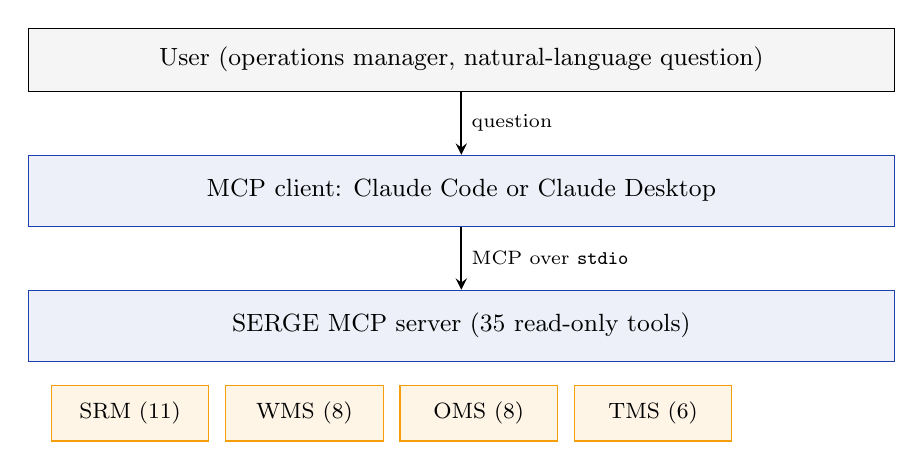
\begin{tikzpicture}[
        node distance=0.8cm,
        layer/.style={rectangle, draw=scblue, fill=scblue!8, minimum width=11cm, minimum height=0.9cm, align=center, font=\small},
        user/.style={rectangle, draw, fill=lightgray, minimum width=11cm, minimum height=0.8cm, align=center, font=\small},
        ctx/.style={rectangle, draw=scaccent, fill=scaccent!10, minimum width=2.0cm, minimum height=0.7cm, align=center, font=\footnotesize},
        arrow/.style={->, thick, >=stealth}
    ]
        \node[user]  (user)   {User (operations manager, natural-language question)};
        \node[layer, below=of user]   (client) {MCP client: Claude Code or Claude Desktop};
        \node[layer, below=of client] (server) {SERGE MCP server (35 read-only tools)};

        \node[ctx, below=0.3cm of server.south west, xshift=1.3cm] (srm) {SRM (11)};
        \node[ctx, right=0.2cm of srm] (wms) {WMS (8)};
        \node[ctx, right=0.2cm of wms] (oms) {OMS (8)};
        \node[ctx, right=0.2cm of oms] (tms) {TMS (6)};

        \draw[arrow] (user)   -- node[right,font=\scriptsize]{question} (client);
        \draw[arrow] (client) -- node[right,font=\scriptsize]{MCP over \texttt{stdio}} (server);
    \end{tikzpicture}
    \caption{The three-layer stack. The user speaks natural language to their desktop client; the client runs SERGE as an MCP subprocess; the server exposes 35 read-only tools grouped by the four systems.}
    \label{fig:stack}
\end{figure}

\section{Agent Layer}

Any \gls{mcp}-compatible client can be used; we run Claude Code. The agent receives the user's question together with a project-level system prompt (\texttt{CLAUDE.md}) that describes the business, enumerates every entity and status, states the critical business rules (refrigerated products require refrigerated carriers; overdue = past required date and not delivered or cancelled), and lists common cross-system reasoning patterns. A final block of \emph{Rules to Avoid Mistakes} (added in the refinement cycle of Chapter~\ref{ch:results}) instructs the agent to never invent identifiers, to distinguish active from historical data, and to list all matching items rather than a subset.

\section{MCP Layer}

The 35 tools are grouped by system and distributed as shown in Table~\ref{tab:toolcount}. All tools are read-only \emph{at the protocol level}: no mutation tool is registered, so the agent cannot write to the backend even if prompted to. Tool descriptions follow Anthropic's guidance~\cite{anthropic2025writingtools}: each states what the tool returns, what its parameters expect, and---for critical tools---an example value. Description quality was re-reviewed between the two evaluation passes; small tightenings on ambiguous tools measurably improved tool-selection accuracy.

\begin{table}[H]
    \centering\small
    \begin{tabularx}{\textwidth}{|l|c|X|}
        \hline
        \rowcolor{lightgray}
        \textbf{System} & \textbf{Tools} & \textbf{Examples} \\
        \hline
        SRM & 11 & \texttt{get\_supplier}, \texttt{compare\_suppliers}, \texttt{list\_supplier\_orders\_by\_status} \\
        \hline
        WMS & 8  & \texttt{check\_inventory}, \texttt{list\_low\_stock}, \texttt{get\_stock\_movements} \\
        \hline
        OMS & 8  & \texttt{get\_customer\_order}, \texttt{search\_customer\_orders\_by\_product} \\
        \hline
        TMS & 6  & \texttt{get\_shipment}, \texttt{track\_customer\_order}, \texttt{list\_exception\_shipments} \\
        \hline
    \end{tabularx}
    \caption{35 MCP tools distributed by system. Full reference in Appendix~\ref{app:tools}.}
    \label{tab:toolcount}
\end{table}

\section{End-to-End Example}

For the question \emph{Why has order ORD-007 not shipped yet?}, a typical run is four tool calls: \texttt{get\_customer\_order} (order is processing), \texttt{track\_customer\_order} (no shipment exists), \texttt{check\_inventory} (8 units on hand against 50 required), \texttt{list\_supplier\_orders\_by\_status} (incoming \gls{po} arrives after the required date). The agent then synthesises the causal chain. No component in the backend is aware the question is diagnostic; the intelligence lives entirely in the agent, which is why swapping \gls{mcp} clients requires no backend change.

% ============================================================================
% CHAPTER 6 — EVALUATION METHODOLOGY
% ============================================================================

\chapter{Evaluation Methodology}
\label{ch:methodology}

\section{Three-Stage Pipeline}

Each scenario is run three times through a three-stage pipeline. The \textbf{agent run} sends the question to Claude Code with the 35 \gls{mcp} tools enabled and captures the response, the tool trace, the duration, and the cost. The \textbf{judge run} sends the agent response plus the scenario's ground truth to a separate \gls{llm} (also Claude Sonnet) with a structured rubric, which returns per-dimension scores, a pass flag, and a failure category. The \textbf{aggregation} step (Python) produces per-scenario, per-level, per-use-case, and failure-taxonomy statistics. The pipeline is resumable: transient failures are retried with exponential back-off, and quota exhaustion is detected explicitly so a run can be continued in a later session.

\section{Judge Rubric: Flexible on Form, Strict on Facts}

Naive \gls{llm}-as-judge setups over-penalise presentation. In our baseline run, one scenario scored 4.18/5.0 on the weighted dimensions but was marked failing because one item of the critical list was not literally mentioned, despite the agent's conclusion being identical to the expected one. The refined judge prompt is organised around one principle: \emph{flexible on form, strict on facts}. Wording variations, alternative tool paths, extra analysis, and answers that extend the ground truth with legitimate data are accepted; wrong values, wrong identifiers, and genuine fabrication are penalised. Identifiers that match the known patterns (\texttt{ORD-XXX}, \texttt{PO-XXX}, \ldots) are not flagged as hallucinations unless they contradict the ground truth.

\section{Complexity Levels}

\begin{table}[H]
    \centering\small
    \begin{tabularx}{\textwidth}{|l|l|c|c|X|}
        \hline
        \rowcolor{lightgray}
        \textbf{Level} & \textbf{Name} & \textbf{N} & \textbf{Tools} & \textbf{Tests} \\
        \hline
        L1 & Trivial   & 4  & 1    & Single entity lookup \\ \hline
        L2 & Simple    & 6  & 1--2 & One-system filter or aggregation \\ \hline
        L3 & Moderate  & 6  & 2--3 & Cross-reference between two systems \\ \hline
        L4 & Complex   & 6  & 3--5 & Causal reasoning across 3--4 systems \\ \hline
        L5 & Expert    & 5  & 6+   & Full diagnostic plus actionable recommendation \\ \hline
    \end{tabularx}
    \caption{Five complexity levels. Complexity is orthogonal to the business use case; each scenario is tagged with both.}
    \label{tab:levels}
\end{table}

\section{Scoring and Metrics}

The judge rates each response on four 1-to-5 dimensions with weights in Table~\ref{tab:dimensions}. A run \textbf{passes} if the weighted score is $\geq$3.5 \emph{and} all critical facts are present \emph{and} no hallucination is detected.

\begin{table}[H]
    \centering\small
    \begin{tabularx}{\textwidth}{|l|r|X|}
        \hline
        \rowcolor{lightgray}
        \textbf{Dimension} & \textbf{Weight} & \textbf{Rewards} \\
        \hline
        Factual accuracy  & 40\% & All values, IDs, dates, statuses match. \\ \hline
        Completeness      & 30\% & Critical facts present. \\ \hline
        No hallucination  & 20\% & No fabricated content. \\ \hline
        Reasoning         & 10\% & Internal coherence. \\ \hline
    \end{tabularx}
    \caption{Judge scoring dimensions.}
    \label{tab:dimensions}
\end{table}

The aggregator also computes the \emph{pass rate}, \emph{functional consistency} (conclusion matches ground truth across repeated runs), the \emph{hallucination rate}, \emph{system coverage} (expected systems actually queried), \emph{tool efficiency} (expected min / actual tool count), and the \emph{measured agent resolution time} per run. Each judge output records a \emph{failure category} from \{\texttt{none}, \texttt{missed\_fact}, \texttt{wrong\_value}, \texttt{hallucination}, \texttt{bad\_reasoning}, \texttt{refused}\}, which powers the failure analysis in Chapter~\ref{ch:results}.

\section{Setup}

Each pass is 27 scenarios $\times$ 3 runs = 81 evaluations. Both agent and judge run on Claude Sonnet. Two passes are reported: \textbf{Run~1} (baseline, 17~April~2026) and \textbf{Run~2} (refined, 18~April~2026, after the iteration cycle documented in \S\ref{sec:finetuning}).

% ============================================================================
% CHAPTER 7 — SCENARIOS
% ============================================================================

\chapter{Scenarios}
\label{ch:scenarios}

\section{Structure}

Each scenario is a JSON document with a natural-language question and a tiered ground truth: \textbf{critical} facts must all appear for the run to pass; \textbf{important} facts are expected but not pass-critical; \textbf{must-not-contain} facts are hard negatives the answer must avoid. Metadata fields (expected systems, minimum tool count, estimated human minutes) drive the aggregator's coverage, efficiency, and time-savings metrics.

\section{The 27 Scenarios}

The scenarios span five business use cases: UC-1 order status, UC-2 root cause, UC-3 supplier/sourcing, UC-4 operational monitoring, UC-5 planning. Use case and complexity level are orthogonal.

\begin{table}[H]
    \centering\scriptsize
    \begin{tabularx}{\textwidth}{|l|l|l|X|}
        \hline
        \rowcolor{lightgray}
        \textbf{ID} & \textbf{Level} & \textbf{UC} & \textbf{Title} \\
        \hline
        L1-01 & L1 & UC-4 & Product Lookup \\ \hline
        L1-02 & L1 & UC-4 & Customer Lookup \\ \hline
        L1-03 & L1 & UC-3 & Supplier Profile \\ \hline
        L1-04 & L1 & UC-4 & List Carriers \\ \hline
        L2-01 & L2 & UC-1 & Basic Order Status \\ \hline
        L2-02 & L2 & UC-4 & Customer Order History \\ \hline
        L2-03 & L2 & UC-4 & Overdue Orders \\ \hline
        L2-04 & L2 & UC-4 & Low Stock Alert \\ \hline
        L2-05 & L2 & UC-3 & Supplier Order History \\ \hline
        L2-06 & L2 & UC-4 & Shipment Exceptions \\ \hline
        L3-01 & L3 & UC-1 & Order Tracking with Current Location \\ \hline
        L3-02 & L3 & UC-4 & Product Demand View \\ \hline
        L3-03 & L3 & UC-3 & Supplier Side-by-Side Comparison \\ \hline
        L3-04 & L3 & UC-3 & Sourcing Options \\ \hline
        L3-05 & L3 & UC-1 & Late Delivery Check \\ \hline
        L3-06 & L3 & UC-4 & Product With Current Inventory \\ \hline
        L4-01 & L4 & UC-2 & Order Delay Diagnosis \\ \hline
        L4-02 & L4 & UC-2 & Carrier Mismatch Diagnosis \\ \hline
        L4-03 & L4 & UC-3 & Supplier Reliability Pattern \\ \hline
        L4-04 & L4 & UC-4 & Operational Scan \\ \hline
        L4-05 & L4 & UC-2 & Customer Impact Assessment \\ \hline
        L4-06 & L4 & UC-1 & Split Shipment Status \\ \hline
        L5-01 & L5 & UC-4 & Full Product Supply Chain History \\ \hline
        L5-02 & L5 & UC-4 & Full Operational Health Check \\ \hline
        L5-03 & L5 & UC-5 & Fulfillment Feasibility Plan \\ \hline
        L5-04 & L5 & UC-3 & Sourcing Strategy Review \\ \hline
        L5-05 & L5 & UC-5 & Reorder Point Analysis \\ \hline
    \end{tabularx}
    \caption{The 27 evaluation scenarios. Full metadata in Appendix~\ref{app:scenarios}.}
    \label{tab:scenarios}
\end{table}

\section{One Scenario per Level}

\textbf{L1-01 Product Lookup.} ``\emph{Tell me about PROD-001}.'' One \gls{wms} call; the agent must pick the right tool on the first try.

\textbf{L2-04 Low Stock Alert.} ``\emph{What products are below their reorder point?}'' One \gls{wms} call; the agent must return all three low-stock products, not a subset.

\textbf{L3-01 Order Tracking.} ``\emph{Where is ORD-005 right now?}'' \gls{oms} then \gls{tms}; the agent synthesises carrier, current location, and ETA from two systems.

\textbf{L4-01 Order Delay Diagnosis.} ``\emph{Why has ORD-007 not shipped?}'' The canonical cross-system diagnostic: \gls{oms} (processing) $\to$ \gls{tms} (no shipment) $\to$ \gls{wms} (stock shortage) $\to$ \gls{srm} (incoming \gls{po} arrives too late).

\textbf{L5-02 Operational Health Check.} ``\emph{Full health check of the supply chain.}'' Scan all four systems, surface overdue orders, exceptions, low stock, supplier reliability concerns; produce at least one cross-system insight.

\section{Ground-Truth Construction}

Ground truths are derived from the scenario data (identifiers below~100). The baseline set was written against scenario data only, which caused the judge to flag legitimate extensions to generated data as hallucinations. The refinement cycle (Chapter~\ref{ch:results}) either rewrote the ground truths to focus on the \emph{shape} of the expected answer rather than exhaustive ID lists, or tightened the judge prompt to accept legitimate extensions.

% ============================================================================
% CHAPTER 8 — RESULTS
% ============================================================================

\chapter{Results}
\label{ch:results}

Two evaluation passes were run: a baseline (\textbf{Run~1}) and a refined pass (\textbf{Run~2}) after one iteration cycle. Run~1 completed 80 of 81 evaluations (one L5 run hit the initial \$0.50 per-run ceiling); Run~2, with the ceiling raised to \$1.50, completed all 81.

\section{Headline Metrics}

\begin{figure}[H]
    \centering
    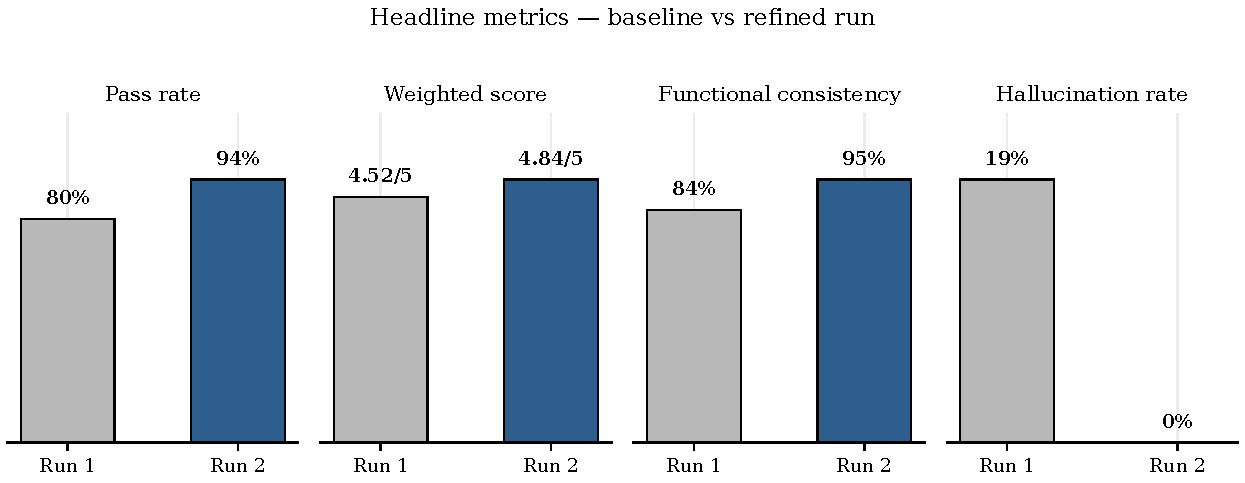
\includegraphics[width=\textwidth]{figures/metrics_dashboard.pdf}
    \caption{Headline metrics. Run~1 (grey) vs Run~2 (blue). Every dimension improves; hallucination rate drops to zero.}
    \label{fig:dashboard}
\end{figure}

Pass rate: 80\% $\to$ 94\%. Weighted score: 4.52 $\to$ 4.84 out of 5.0. Functional consistency: 84\% $\to$ 95\%. Hallucination rate: 19\% $\to$ \textbf{0\%}. The refined agent fabricates nothing across 81 runs.

\begin{tcolorbox}[colback=scblue!4, colframe=scblue!60, fonttitle=\bfseries, title=Result,
    boxrule=0.5pt, arc=2pt, left=6pt, right=6pt, top=3pt, bottom=3pt]
Across 81 refined evaluations: \textbf{94\% pass rate}, \textbf{4.84/5.0} weighted score, \textbf{zero fabricated data}.
\end{tcolorbox}

\section{Refinement Cycle}
\label{sec:finetuning}

Three changes between the two passes account for the improvement.

\textbf{Ground-truth recalibration.} Five scenarios in Run~1 passed at 0\% despite high underlying scores. Inspection showed the ground truths listed scenario-only identifiers while the agent correctly used the full dataset, and the judge flagged the extensions as hallucinations. Four were rewritten to focus on answer shape; one had a single over-strict critical fact demoted to important.

\textbf{Judge prompt revision.} An explicit rule was added: identifiers matching the domain patterns are not hallucinations unless they contradict the ground truth. The \texttt{hallucination} failure category is now reserved for genuine fabrication (names outside the domain, impossible values, contradictions).

\textbf{Agent prompt revision.} A \emph{Rules to Avoid Mistakes} section was added to the agent's system prompt: never invent identifiers, distinguish active from historical data, list all matching items, compute metrics over the full result set, respect the critical business rules on cold chain and reorder points.

\section{By Complexity Level}

\begin{figure}[H]
    \centering
    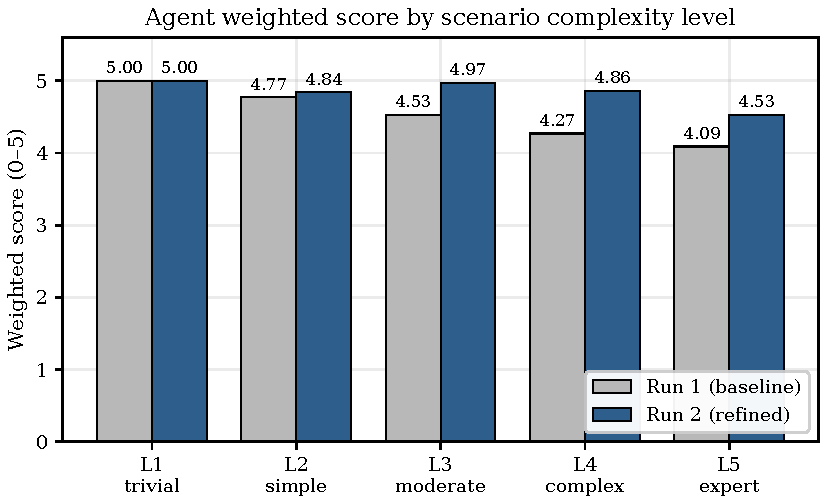
\includegraphics[width=0.92\textwidth]{figures/score_by_level.pdf}
    \caption{Weighted score by complexity level.}
    \label{fig:score_level}
\end{figure}

Accuracy decreases with complexity, as expected, but flattens in Run~2. L1 stays at 5.0. L3 rises 4.53 $\to$ 4.97. \textbf{L4 rises 4.27 $\to$ 4.86 and passes at 100\%}---the canonical cross-system diagnostics all succeed. L5 rises 4.09 $\to$ 4.53 and remains the hardest level.

\section{By Use Case}

\begin{figure}[H]
    \centering
    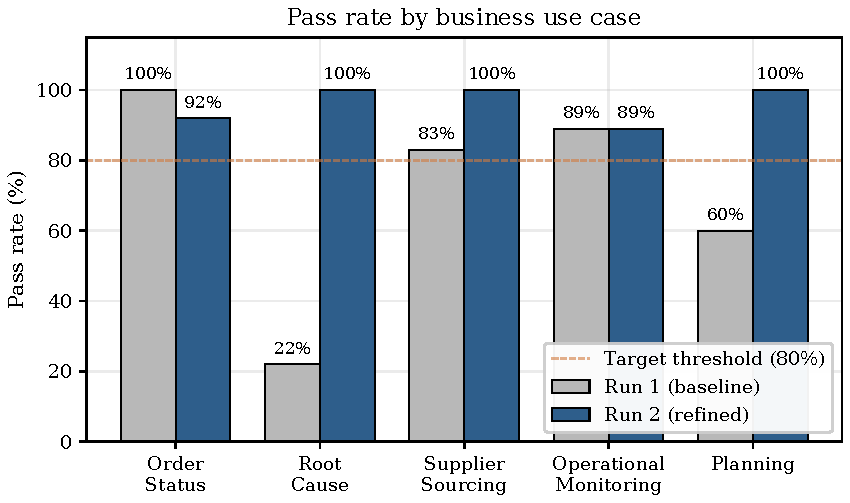
\includegraphics[width=0.92\textwidth]{figures/pass_rate_by_uc.pdf}
    \caption{Pass rate by business use case.}
    \label{fig:pass_uc}
\end{figure}

UC-2 (Root Cause) rises from 22\% to 100\%---the largest shift. UC-3 and UC-5 also reach 100\%. UC-4 stays at 89\%. UC-1 regresses marginally (100\% $\to$ 92\%) because of one partial L2 answer, which does not affect the aggregate.

\section{Failure Taxonomy}

\begin{figure}[H]
    \centering
    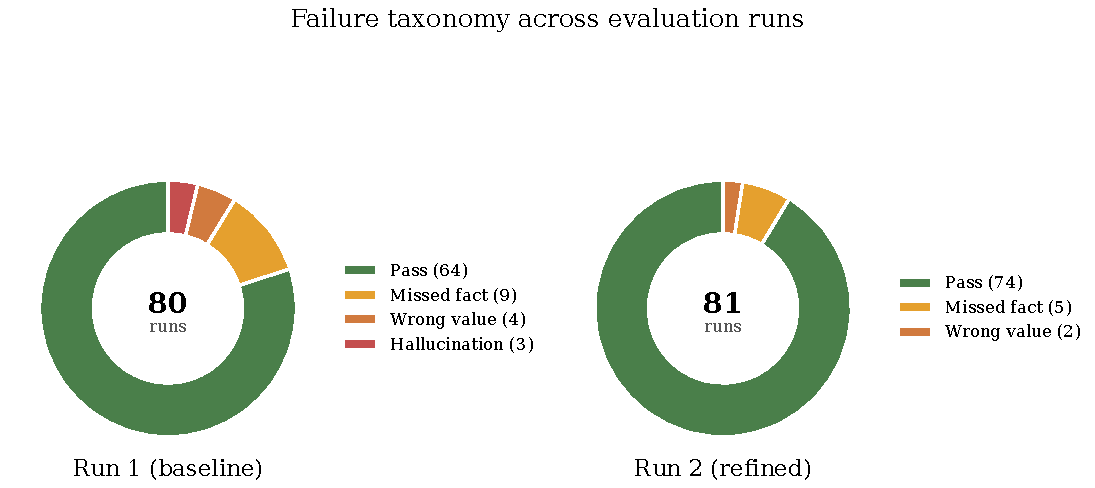
\includegraphics[width=\textwidth]{figures/failure_taxonomy.pdf}
    \caption{Failure taxonomy for both passes.}
    \label{fig:failures}
\end{figure}

\texttt{hallucination} falls from 4\% to 0\%, \texttt{wrong\_value} from 5\% to 2\%, \texttt{missed\_fact} from 11\% to 6\%. The zero-hallucination outcome is the combined effect of the agent rule (never invent) and the judge rule (no false positive on legitimate extensions).

\section{Resolution Time}

\begin{figure}[H]
    \centering
    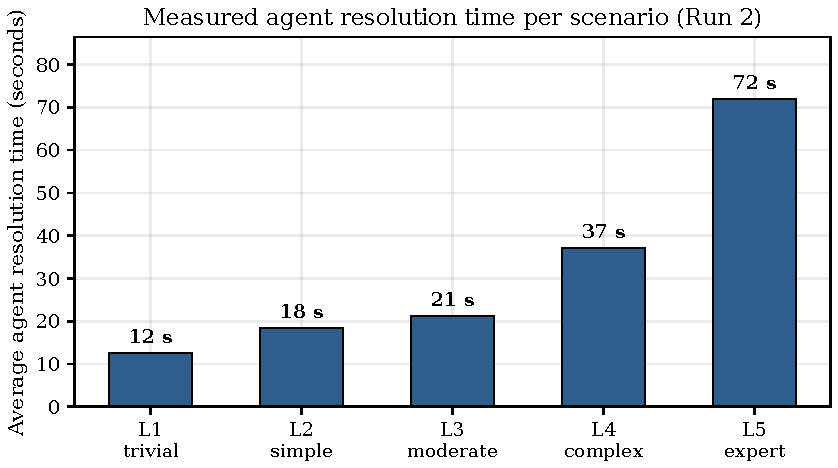
\includegraphics[width=\textwidth]{figures/time_savings.pdf}
    \caption{Measured agent resolution time per complexity level (Run~2).}
    \label{fig:time}
\end{figure}

Measured averages per scenario: L1 $\approx$ 13\,s, L2 $\approx$ 18\,s, L3 $\approx$ 21\,s, L4 $\approx$ 37\,s, L5 $\approx$ 72\,s. Across the 81 Run~2 evaluations the agent spent 43.5\,min in total, averaging about 32\,s per run.

\section{Cross-System Coverage}

\begin{figure}[H]
    \centering
    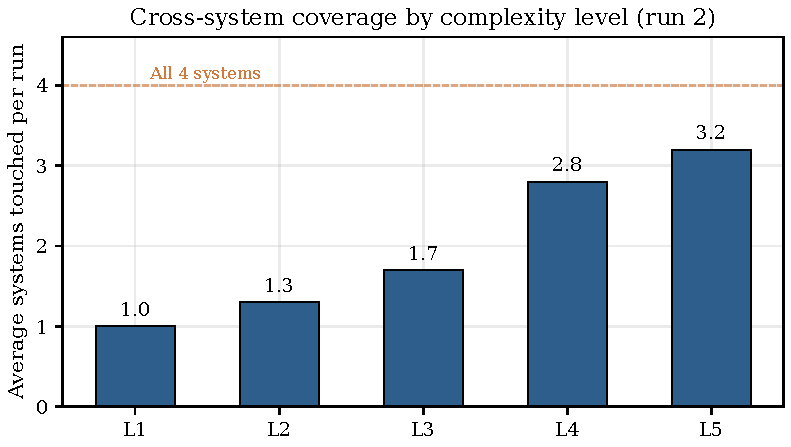
\includegraphics[width=0.85\textwidth]{figures/systems_touched.pdf}
    \caption{Average systems touched per run, by level (Run~2).}
    \label{fig:coverage}
\end{figure}

L1 averages 1 system; L4 averages 2.8; L5 averages 3.2. The agent does chain across systems when the question requires it, and stays scoped when it does not.

\section{Qualitative Behaviour}

Three Run~2 responses illustrate behaviour that scalar metrics do not fully capture. On the carrier-mismatch diagnosis, the agent identifies the storage-type mismatch, references the \texttt{SHP-009} refrigeration failure as evidence, and lists refrigerated alternatives---a production-quality incident report. On the full product history, the agent chains six tool calls, computes a running stock balance from movements, produces an ASCII flow diagram, and ends with a two-sentence takeaway. On the fulfilment-feasibility question, it computes the 4-unit gap, compares the two refrigerated carriers, and proposes three options with trade-offs.

% ============================================================================
% CHAPTER 9 — DISCUSSION
% ============================================================================

\chapter{Discussion}
\label{ch:discussion}

\section{What Worked}

\textbf{MCP delivered on its agent-agnostic promise.} The same backend runs unchanged under Claude Code and Claude Desktop; any \gls{mcp}-compatible client would work without modification.

\textbf{Flexible-on-form judging lifted the pass rate by 14 points.} The most impactful methodological change between the two runs was the judge rubric, not the agent. The agent was already correct in most scenarios that failed Run~1.

\textbf{Tool descriptions and system prompt are the high-leverage artefacts.} The iteration budget was spent on these two surfaces, not on code. The measured accuracy improvement between Run~1 and Run~2 came almost entirely from prompt-level changes.

\section{Limitations}

The dataset is simulated and contains patterns we designed; a production dataset would include noise and edge cases not exercised here. The domain is narrow (one small distributor in Bangkok), so generalisation across verticals is untested. Both agent and judge are Claude Sonnet, so cross-family comparison is left to future work. The judge is itself an \gls{llm}, and is not cross-validated against humans.

\section{Threats to Validity}

A critic could argue that the Run~1 $\to$ Run~2 improvement is partly due to ground-truth softening. Three observations push back. First, the hallucination rate---a purely factual metric independent of rubric tolerance---fell from 19\% to 0\%. Second, functional consistency rose from 84\% to 95\% and measures whether the conclusion is correct, not whether a list of facts is matched. Third, L1 and L2 scenarios, none of which had their ground truths modified, also improved marginally between runs. The ground-truth recalibration explains part of the L3--L4 improvement but not the hallucination and consistency gains.

We report \emph{measured} agent resolution times (13--72\,s per scenario, averaging 32\,s per run) but do not claim a percentage saving over a human. Comparing against a human baseline would require measured data from real operators, which we do not have.

\section{Implications for Practice}

Three practical implications. \textbf{Read-only is a defensible initial scope}: the diagnostic value alone justifies the deployment, and write access can be added later once trust is established. \textbf{\gls{mcp} integration is cheap insurance}: the investment is small and preserves optionality on the agent side. \textbf{Tool descriptions and the system prompt deserve explicit ownership}, as much as the data model itself; both dominate the measured agent accuracy.

% ============================================================================
% CHAPTER 10 — CONCLUSION
% ============================================================================

\chapter{Conclusion}
\label{ch:conclusion}

SERGE is a read-only AI agent connecting four supply chain systems through the \gls{mcp}. Over a simulated B2B mango distributor in Bangkok, and evaluated on 27 scenarios spanning five complexity levels, the refined pass reaches a 94\% pass rate, a 4.84/5.0 weighted score, zero hallucinations across 81 evaluations, and 95\% functional consistency. Measured agent resolution time averages 13\,s on trivial scenarios and 72\,s on expert-level ones.

Four contributions follow. A plug-and-play \gls{mcp} architecture for supply chain systems, agent-agnostic by design. A read-only diagnostic agent pattern, complementary to the optimisation-centric literature. A flexible \gls{llm}-as-judge methodology with a structured failure taxonomy, validated through an explicit iteration cycle. A reusable benchmark of 27 scenarios released with the work.

Three directions extend this naturally: a predictive layer for demand and disruption forecasting; controlled write access behind a human-in-the-loop approval workflow; and a cross-agent comparison holding the \gls{mcp} backend and the scenarios fixed. We leave these to future work.


% ── References ───────────────────────────────────────────────────────
% ============================================================================
% REFERENCES (as a chapter)
% ============================================================================
\chapter*{References}
\addcontentsline{toc}{chapter}{References}

\begin{thebibliography}{99}

\bibitem{vaswani2017attention}
A.~Vaswani, N.~Shazeer, N.~Parmar, J.~Uszkoreit, L.~Jones, A.~N. Gomez, \L.~Kaiser, and I.~Polosukhin. Attention is all you need. \emph{Advances in Neural Information Processing Systems}, 30:5998--6008, 2017.

\bibitem{kaplan2020scaling}
J.~Kaplan, S.~McCandlish, T.~Henighan, T.~B. Brown, B.~Chess, R.~Child, S.~Gray, A.~Radford, J.~Wu, and D.~Amodei. Scaling laws for neural language models. \emph{arXiv:2001.08361}, 2020.

\bibitem{hoffmann2022chinchilla}
J.~Hoffmann, S.~Borgeaud, A.~Mensch, et~al. Training compute-optimal large language models. \emph{arXiv:2203.15556}, 2022.

\bibitem{wei2022emergent}
J.~Wei, Y.~Tay, R.~Bommasani, et~al. Emergent abilities of large language models. \emph{Transactions on Machine Learning Research}, 2022.

\bibitem{yao2023react}
S.~Yao, J.~Zhao, D.~Yu, N.~Du, I.~Shafran, K.~Narasimhan, and Y.~Cao. ReAct: Synergizing reasoning and acting in language models. In \emph{Proceedings of ICLR}, 2023.

\bibitem{schick2023toolformer}
T.~Schick, J.~Dwivedi-Yu, R.~Dess\`i, R.~Raileanu, M.~Lomeli, L.~Zettlemoyer, N.~Cancedda, and T.~Scialom. Toolformer: Language models can teach themselves to use tools. In \emph{Proceedings of NeurIPS}, 2023.

\bibitem{weng2023agents}
L.~Weng. LLM powered autonomous agents. \url{https://lilianweng.github.io/posts/2023-06-23-agent/}, 2023.

\bibitem{patil2024gorilla}
S.~G. Patil, T.~Zhang, X.~Wang, and J.~E. Gonzalez. Gorilla: Large language model connected with massive APIs. In \emph{Proceedings of NeurIPS}, 2024.

\bibitem{anthropic2024agents}
Anthropic. Building effective agents. \url{https://www.anthropic.com/research/building-effective-agents}, 2024.

\bibitem{anthropic2025howccworks}
Anthropic. How Claude Code works. \url{https://code.claude.com/docs/en/how-claude-code-works}, 2025.

\bibitem{anthropic2025contextengineering}
Anthropic. Effective context engineering for AI agents. \url{https://www.anthropic.com/engineering/effective-context-engineering-for-ai-agents}, 2025.

\bibitem{anthropic2025writingtools}
Anthropic. Writing tools for agents. \url{https://www.anthropic.com/engineering/writing-tools-for-agents}, 2025.

\bibitem{mcp2024}
Anthropic. Model context protocol. \url{https://www.anthropic.com/news/model-context-protocol}, 2024.

\bibitem{mcpspec}
Model context protocol specification (2025-11-25). \url{https://modelcontextprotocol.io/specification/2025-11-25}, 2025.

\bibitem{geodis2024}
GEODIS. Supply chain visibility survey. Cited by Descartes Systems, 2024.

\bibitem{aws2024sync}
Synchronizing ERP, WMS, and TMS systems for supply chain optimization. \emph{Supply \& Demand Chain Executive / AWS}, 2024.

\bibitem{omniful2026}
Omniful. Unified dashboard: Connecting ERP, OMS, WMS, and TMS, 2026.

\bibitem{jannelli2024agentic}
V.~Jannelli, S.~Schoepf, M.~Bickel, T.~Netland, and A.~Brintrup. Agentic LLMs in the supply chain: Towards autonomous multi-agent consensus-seeking. \emph{International Journal of Production Research}, 2025.

\bibitem{yin2025scpa}
J.~Yin et~al. Rethinking supply chain planning: A generative paradigm (SCPA). \emph{arXiv:2509.03811}, 2025.

\bibitem{almahri2026disruption}
S.~AlMahri, L.~Xu, and A.~Brintrup. Automating supply chain disruption monitoring via an agentic AI approach. \emph{arXiv:2601.09680}, 2026.

\bibitem{zhang2025rag}
Y.~Zhang et~al. Multi-agent RAG for supply chain knowledge bases. In \emph{KDD 2025 Workshop}, 2025.

\bibitem{gaisc2025systematic}
Systematic analysis of generative AI for supply chain transformation. \emph{ScienceDirect}, 2025.

\bibitem{zheng2023judge}
L.~Zheng, W.-L. Chiang, Y.~Sheng, et~al. Judging LLM-as-a-judge with MT-bench and chatbot arena. In \emph{Proceedings of NeurIPS}, 2023.

\bibitem{gu2024judgesurvey}
J.~Gu et~al. A survey on LLM-as-a-judge. \emph{arXiv:2411.15594}, 2024.

\bibitem{li2024judgessurvey}
H.~Li et~al. LLMs-as-judges: A comprehensive survey on LLM-based evaluation methods. \emph{arXiv:2412.05579}, 2024.

\bibitem{shankar2024validators}
S.~Shankar et~al. Who validates the validators? Aligning LLM-assisted evaluation with human preferences. \emph{arXiv:2404.12272}, 2024.

\bibitem{evans2003ddd}
E.~Evans. \emph{Domain-Driven Design: Tackling Complexity in the Heart of Software}. Addison-Wesley, 2003.

\end{thebibliography}


% ── Appendices ───────────────────────────────────────────────────────
\appendix
% ============================================================================
% APPENDIX A — MCP TOOL REFERENCE
% ============================================================================

\chapter{MCP Tool Reference}
\label{app:tools}

The 35 \gls{mcp} tools are listed below. Naming convention: \texttt{\textit{system}\_\textit{verb}\_\textit{noun}}. All tools are read-only.

{\footnotesize
\begin{longtable}{@{}p{6.2cm}p{8.5cm}@{}}
\toprule
\textbf{Tool} & \textbf{Description} \\
\midrule
\endfirsthead
\toprule
\textbf{Tool} & \textbf{Description} \\
\midrule
\endhead
\multicolumn{2}{@{}l}{\textbf{SRM --- Procurement}} \\
\addlinespace[2pt]
\texttt{srm\_get\_supplier} & Supplier profile. \\
\texttt{srm\_list\_suppliers} & All suppliers. \\
\texttt{srm\_get\_supplier\_product} & One supplier-product entry (cost, product link). \\
\texttt{srm\_list\_supplier\_products\_by\_supplier} & All items offered by one supplier. \\
\texttt{srm\_list\_supplier\_products\_by\_product} & All suppliers that sell a given product. \\
\texttt{srm\_get\_supplier\_order} & One supplier order by ID. \\
\texttt{srm\_list\_all\_supplier\_orders} & All supplier orders. \\
\texttt{srm\_list\_supplier\_orders\_by\_supplier} & Supplier orders placed with a given supplier. \\
\texttt{srm\_list\_supplier\_orders\_by\_status} & Supplier orders filtered by status. \\
\texttt{srm\_list\_overdue\_supplier\_orders} & Supplier orders past expected delivery. \\
\texttt{srm\_compare\_suppliers} & Side-by-side supplier performance. \\
\addlinespace[4pt]
\multicolumn{2}{@{}l}{\textbf{WMS --- Inventory}} \\
\addlinespace[2pt]
\texttt{wms\_get\_product} & Product by ID. \\
\texttt{wms\_get\_product\_by\_sku} & Product by SKU. \\
\texttt{wms\_list\_products} & All products. \\
\texttt{wms\_check\_inventory} & Inventory status for one product. \\
\texttt{wms\_list\_low\_stock} & Products below reorder point. \\
\texttt{wms\_get\_stock\_movements} & Movement history for one product. \\
\texttt{wms\_list\_all\_inventory} & Full inventory snapshot. \\
\texttt{wms\_get\_warehouse} & Warehouse by ID. \\
\addlinespace[4pt]
\multicolumn{2}{@{}l}{\textbf{OMS --- Sales}} \\
\addlinespace[2pt]
\texttt{oms\_get\_customer\_order} & Customer order with line items. \\
\texttt{oms\_get\_customer} & Customer by ID. \\
\texttt{oms\_list\_customer\_orders\_by\_customer} & Customer orders for one customer. \\
\texttt{oms\_list\_customer\_orders\_by\_status} & Customer orders filtered by status. \\
\texttt{oms\_list\_overdue\_customer\_orders} & Customer orders past required date. \\
\texttt{oms\_list\_all\_customer\_orders} & All customer orders. \\
\texttt{oms\_list\_customers} & All customers. \\
\texttt{oms\_search\_customer\_orders\_by\_product} & Customer orders containing a product. \\
\addlinespace[4pt]
\multicolumn{2}{@{}l}{\textbf{TMS --- Shipping}} \\
\addlinespace[2pt]
\texttt{tms\_get\_shipment} & Shipment with tracking events. \\
\texttt{tms\_track\_customer\_order} & All shipments for a customer order. \\
\texttt{tms\_list\_exception\_shipments} & Shipments in exception state. \\
\texttt{tms\_get\_carrier} & Carrier by ID. \\
\texttt{tms\_list\_shipments\_by\_status} & Shipments filtered by status. \\
\texttt{tms\_list\_carriers} & All carriers. \\
\bottomrule
\end{longtable}
}

% ============================================================================
% APPENDIX B: SCENARIO METADATA
% ============================================================================

\chapter{Scenario Metadata}
\label{app:scenarios}

Table~\ref{tab:scenariosmeta} lists all 27 scenarios with their expected system coverage, minimum tool count, and human-baseline estimate. These metadata fields are used by the aggregator to compute cross-system coverage, tool efficiency, and time-savings metrics.

\begin{longtable}{@{}llllrr@{}}
\caption{Scenario metadata.}\label{tab:scenariosmeta}\\
\toprule
\textbf{ID} & \textbf{Level} & \textbf{UC} & \textbf{Expected systems} & \textbf{Min tools} & \textbf{Human min} \\
\midrule
\endfirsthead
\toprule
\textbf{ID} & \textbf{Level} & \textbf{UC} & \textbf{Expected systems} & \textbf{Min tools} & \textbf{Human min} \\
\midrule
\endhead
L1-01 & L1 & UC-4 & WMS               & 1 & 2  \\
L1-02 & L1 & UC-4 & OMS               & 1 & 2  \\
L1-03 & L1 & UC-3 & SRM               & 1 & 2  \\
L1-04 & L1 & UC-4 & TMS               & 1 & 2  \\
L2-01 & L2 & UC-1 & OMS               & 1 & 5  \\
L2-02 & L2 & UC-4 & OMS               & 1 & 6  \\
L2-03 & L2 & UC-4 & OMS               & 1 & 5  \\
L2-04 & L2 & UC-4 & WMS               & 1 & 5  \\
L2-05 & L2 & UC-3 & SRM               & 1 & 6  \\
L2-06 & L2 & UC-4 & TMS               & 1 & 5  \\
L3-01 & L3 & UC-1 & OMS, TMS          & 2 & 10 \\
L3-02 & L3 & UC-4 & WMS, OMS          & 2 & 12 \\
L3-03 & L3 & UC-3 & SRM               & 1 & 15 \\
L3-04 & L3 & UC-3 & SRM               & 1 & 10 \\
L3-05 & L3 & UC-1 & OMS, TMS          & 2 & 8  \\
L3-06 & L3 & UC-4 & WMS               & 1 & 5  \\
L4-01 & L4 & UC-2 & OMS, TMS, WMS, SRM & 4 & 25 \\
L4-02 & L4 & UC-2 & TMS, OMS, WMS     & 3 & 20 \\
L4-03 & L4 & UC-3 & SRM               & 2 & 15 \\
L4-04 & L4 & UC-4 & OMS, TMS, WMS, SRM & 4 & 25 \\
L4-05 & L4 & UC-2 & WMS, OMS          & 3 & 20 \\
L4-06 & L4 & UC-1 & OMS, TMS, WMS     & 3 & 18 \\
L5-01 & L5 & UC-4 & SRM, WMS, OMS     & 6 & 40 \\
L5-02 & L5 & UC-4 & OMS, TMS, WMS, SRM & 6 & 45 \\
L5-03 & L5 & UC-5 & OMS, WMS, SRM, TMS & 6 & 35 \\
L5-04 & L5 & UC-3 & SRM               & 4 & 30 \\
L5-05 & L5 & UC-5 & WMS, OMS, SRM     & 5 & 35 \\
\bottomrule
\end{longtable}


% ── Glossary ─────────────────────────────────────────────────────────
\printglossaries

\end{document}
